\documentclass{article}
\usepackage[utf8]{inputenc}
\usepackage{setspace} 
\usepackage{enumitem}
\usepackage{geometry}
 \geometry{
 a4paper,
 left=30mm,
 right=30mm,
 top=30mm,
 }
%% For directory trees
\usepackage{dirtree}
\usepackage{listings}
\lstset{language=C++}

\title{\textbf{A JUCE Audio Plugin for Distortion Effects}}
\author{Person codes: 10783942, 10561598, 10500756, 10583734, 10472602}
\date{May 2021}


\usepackage[numbers, square, sort]{natbib}
\usepackage{graphicx}
\usepackage{amsmath}
\usepackage{url}
\newcommand{\code}{\texttt}
\usepackage[justification=centering]{caption}

\begin{document}

\maketitle

\section{Introduction}
Distortion effects are very popular among guitarists because of the additional expressiveness that they provide. The key of distortion is always a non-linearity between the input and output signal, which provides additional richness to the guitar sound.\\
This report describes the implementation of several audio distortion effects that are described in Chapter 7 of \cite{reiss2014audio}. The effects are implemented in form of a cross-platform \code{JUCE} \cite{JUCE} audio plugin, written in C++. The source code, as well as pre-compiled binaries, are made available in a dedicated GitHub repository\footnote{\url{https://github.com/magiwanders/CMLS_HW2}}.

\section{Distortion types}
There are different types of non-linearities that are used to create different distortion effects, and our plugin implements seven of them. The following paragraphs provide a short qualitative description for each effect. Please mind that each effect features a post-processing low-pass filter which can soften some of the "hard edges" produced by the methods explained below. 
\paragraph{Hard clipping} 
Hard clipping is achieved by setting a threshold, upon which which the amplitude of the waveform is abruptly clipped. The threshold is symmetrical, since it is equally applied to the negative and positive part of the waveform. The sharp corners of the resulting waveform produce many harmonics and a very rough sound.
\paragraph{Soft clipping}
Unlike hard clipping, soft clipping does not apply the threshold abruptly. The transition between the un-clipped and the clipped region is more smooth, which results in a less harsh sound. 
\paragraph{Exponential soft clipping} 
Exponential soft clipping is a nonlinear compression, obtained by subtracting to each sample a quantity proportional to its value. Distortion is produced by the inverse exponential nature of the compression. 
\paragraph{Full wave rectification} 
Full wave rectification is achieved by reflecting the sound wave over the $x$ axis. This corresponds to making all negative sample values positive.
\paragraph{Half wave rectification} 
Half wave rectification is achieved by canceling any negative half wave, setting to zero any negative sample value. Both full wave and half wave rectification output signals that are no longer zero-mean.
\paragraph{Inter-modulation distortion} 
Inter modulation distortion consists in a "harmonic pollution" of the signal due to a square elevation of the waveform. 
\paragraph{Slew rate distortion}
Slew rate distortion is achieved by limiting the maximum absolute difference between successive samples, effectively "cutting" each fast changing waveform portion with an oblique line. This produces an effect that vaguely resembles analogue artifacts.

%\clearpage
\section{Implementation in JUCE}
The code is divided into the following C++ source files:
\bigskip

%{\fontsize{8pt}{8pt}\selectfont
\dirtree{%
.1 Source/.
.2 PluginEditor.h.
.2 PluginEditor.cpp.
.2 PluginParameters.h.
.2 PluginProcessor.h.
.2 PluginProcessor.cpp.
} % end of dirtree
%} % end of \fontsize

\bigskip
\noindent The \code{PluginEditor} class takes care of the user interface of the plugin. It exposes the parameters that can be modified by the user and updates them constantly.\\
The \code{PluginParameters.h} header contains \code{enum} definitions that make it easier to interpret the identification numbers of distortion types and slider types. This header in shared by the \code{PluginEditor} and \code{PluginProcessor} classes, in order to make the naming consistent.\\
The \code{PluginProcessor} class implements all of the distortion effects and takes care of adjusting them based on the parameters adjusted by the user.


\section{Plugin usage}
The usage of the plugin is very straightforward. There is a different number of parameters for each distortion type. Each parameter can be adjusted by means of a slider, as shown in Figure \ref{fig:parameters_soft}. The parameters are described in the following paragraphs.
\begin{figure}[h!]
\centering
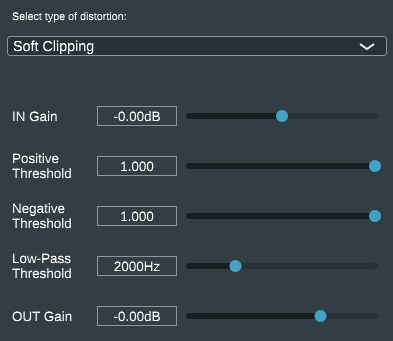
\includegraphics[scale=0.6]{images/cmlshw2_soft.png}
\caption{Adjustable parameters for soft clipping}
\label{fig:parameters_soft}
\end{figure}
\paragraph{Distortion type} The choice of the distortion type is made available in form of a simple combo box, as shown in Figure \ref{fig:dist_type_combobox}. One of the six options can be selected: hard clipping, soft clipping, exponential soft clipping, full-wave rectification, half-wave rectification, intermodulation distortion and slew rate distortion.
\begin{figure}[h!]
\centering
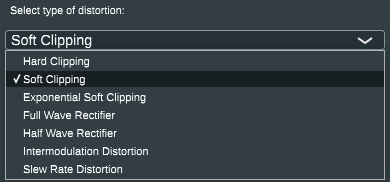
\includegraphics[scale=0.6]{images/cmlshw2_tendina.png}
\caption{Distortion type selection menu}
\label{fig:dist_type_combobox}
\end{figure}
\paragraph{Input gain} The user can control the input gain (dB) by adjusting the slider. The range of values is between -24dB and +24dB.
\paragraph{Clipping threshold \textit{(For hard clipping)}} Hard clipping requires the setting of a threshold, upon or below which the waveform is cut abruptly. This means that the selected threshold acts symmetrically for the positive and the negative amplitude of the waveform.
\paragraph{Positive threshold and negative threshold \textit{(For soft clipping)}} In the case of soft clipping, two thresholds can be set: one for the positive and another for the negative threshold. As the name suggests, the transition between to the clipped waveform is less abrupt than the hard clipping.
\paragraph{Maximum slew rate \textit{(For slew rate distortion)}}
This controls the maximum allowed delta value between successive samples. Mind that this applies for both "increasing" deltas (newest sample greater than previous one) and "descending" deltas.  
\paragraph{Low-pass frequency} This slider controls the cutoff frequency (Hz) of the lowpass filter be in, which is applied after the distortion effect. The LPF is used to soften the sound and selectively reduce the harmonic pollution at the higher frequencies, which can easily be undesirable.
\paragraph{Output gain} This slider controls the gain that is applied after the lowpass filter. This is needed to compensate for possible gain imbalances created by the distortion processing.

\bibliographystyle{unsrt}
\bibliography{references}
\end{document}
